\documentclass{article}
\usepackage{amsmath}
\usepackage{tikz}
\usetikzlibrary{arrows.meta}

\begin{document}

\begin{figure}[h]
    \centering
    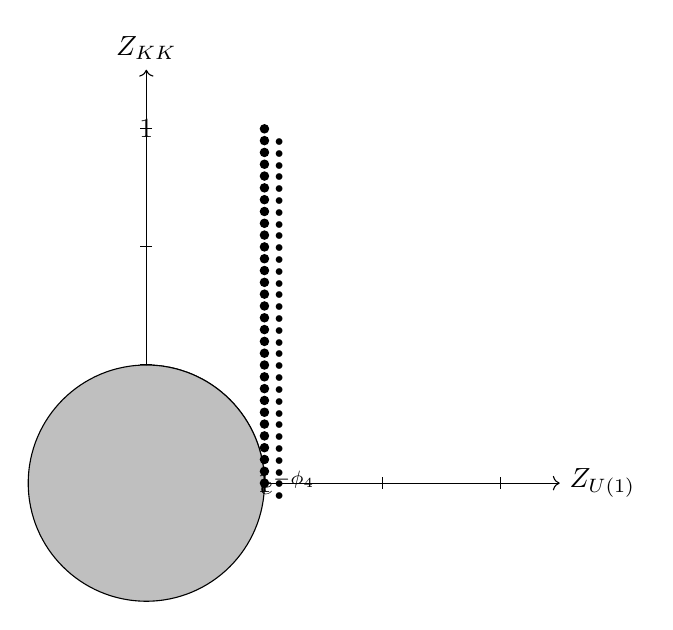
\begin{tikzpicture}[scale=1.5]
        % Axes
        \draw[->] (-0.5,0) -- (3.5,0) node[right] {$Z_{U(1)}$};
        \draw[->] (0,-0.5) -- (0,3.5) node[above] {$Z_{KK}$};
        
        % Grid lines
        \foreach \x in {0,...,3}
            \draw (\x,0.05) -- ++(0,-0.1);
        \foreach \y in {0,...,3}
            \draw (0.05,\y) -- ++(-0.1,0);
        
        % Circle
        \draw[fill=gray!50] (0,0) circle (1cm);
        \draw[fill=gray!50] (1,0) arc (0:90:1);
        
        % Dots
        \foreach \y [count=\i from 1] in {0.1,0.2,...,3}
            \filldraw[black] (1,\y) circle (1pt) node[below right] {\tiny $\bullet$};
        
        % Label for e^(-phi_4)
        \filldraw[black] (1,0) circle (1pt) node[below right] {\tiny $\bullet$};
        \node at (1.2,0) {$e^{-\phi_4}$};
        
        % Labels for axes
        \node at (0,3) {$1$};
        \node at (1,0) {$1$};
    \end{tikzpicture}
    \caption{The 'convex hull' (see \cite{Heidenreich:2015nta} for notation) of gonions and a KK tower in circle compactification, here just the vertical dot line, always contains the extremal circle, if we remain in a perturbative region $e^{-\phi_4}=g^{-1}\geq 1$.}
    \label{fig:convex_hull}
\end{figure}

\end{document}